%
% File emnlp2019.tex
%
%% Based on the style files for ACL 2019, which were
%% Based on the style files for EMNLP 2018, which were
%% Based on the style files for ACL 2018, which were
%% Based on the style files for ACL-2015, with some improvements
%%  taken from the NAACL-2016 style
%% Based on the style files for ACL-2014, which were, in turn,
%% based on ACL-2013, ACL-2012, ACL-2011, ACL-2010, ACL-IJCNLP-2009,
%% EACL-2009, IJCNLP-2008...
%% Based on the style files for EACL 2006 by 
%%e.agirre@ehu.es or Sergi.Balari@uab.es
%% and that of ACL 08 by Joakim Nivre and Noah Smith

\documentclass[11pt,a4paper]{article}
\usepackage[hyperref]{emnlp-ijcnlp-2019}
\usepackage{times}
\usepackage{latexsym}
\usepackage{graphicx}  %%% for including graphics
\usepackage{booktabs}
\usepackage{xspace}
\usepackage{multirow}
\usepackage{url}

%\aclfinalcopy % Uncomment this line for the final submission

%\setlength\titlebox{5cm}
% You can expand the titlebox if you need extra space
% to show all the authors. Please do not make the titlebox
% smaller than 5cm (the original size); we will check this
% in the camera-ready version and ask you to change it back.

\newcommand\BibTeX{B{\sc ib}\TeX}
\newcommand\confname{EMNLP-IJCNLP 2019}
\newcommand\conforg{SIGDAT}
\newcommand{\refexp}[1]{\textsl{#1}}
\newcommand{\word}[1]{\textsl{#1}}
\newcommand{\cat}[1]{\textsc{#1}}
\newcommand{\vgenome}{VisualGenome\xspace}
\newcommand{\ra}{$\rightarrow$}

\newcommand{\sz}[1]{\textcolor{blue}{\emph{//sz: #1//}}}
\newcommand{\gbt}[1]{\textcolor{orange}{\emph{//g: #1//}}}
\newcommand{\cs}[1]{\textcolor{green!60!black}{\emph{//cs: #1//}}}

\title{Supplemental Material for submission ``Do Objects in Real-World Images Have a Canonical Name?''}

\author{First Author \\
  Affiliation / Address line 1 \\
  Affiliation / Address line 2 \\
  Affiliation / Address line 3 \\
  {\tt email@domain} \\\And
  Second Author \\
  Affiliation / Address line 1 \\
  Affiliation / Address line 2 \\
  Affiliation / Address line 3 \\
  {\tt email@domain} \\}

\date{}

\begin{document}
\maketitle
\section{Dataset: Supplementary Information}
\label{app:instructions}

Figures~\ref{fig:instructions1} and \ref{fig:instructions2} contain the instructions for our subjects in the first round and rounds 2-4, respectively.
After the first round, based on the opt-out annotation, we kept images that met all the following conditions (thresholds were estimated via manual inspection):
\begin{itemize}
\item they were not marked as occluded by any subject;
\item ``Bounding box is unclear'' was marked at most twice;
\item at most 17\% of elicited names were in plural form (to remove cases where the bounding box contains several objects);
\item the most frequent elicited name is of the same domain as the \vgenome name.
\end{itemize}
This yielded $25,596$ images, discarding $5,497$.
Table~\ref{tab:overview_dataset2} gives an overview of the collection synsets, grouped into the $7$~domains, and Table~\ref{tab:overview_dataset1} shows the $7$\ domains together with the top $10$\ VG names.
\iffalse
\begin{table*}[t]
	\small
	\centering
 \begin{tabular}{ll@{~}l@{~}l@{~}l@{~}l@{~}l@{~}}
 	\toprule
 	{} &              &                  \\
 	\midrule
 	home           &  bed (888) &  bench (714) &  table (687) &  desk (672) &  counter (516) \\
 	&  couch (366) &  chair (365) &  carpet (307) &  bowl (219) &  curtain (182) \\
 	buildings      &  house (340) &  bridge (274) &  dugout (91) &  tent (53) &  restaurant (33)\\
 	 &  overpass (23) 	&  grill (22) &  garage (18) &  hotel (16) &  castle (14) \\
 	vehicles       &  train (954) &  car (642) &  plane (485) &  airplane (479) &  motorcycle (466) \\
 	 &  truck (465) 	&  boat (450) &  jet (106) &  aircraft (85) &  van (76) \\
 	people         &  boy (853) &  man (806) &  woman (766) &  girl (650) &  lady (342)\\
 	 &  guy (330) &  child (230) &  batter (110) &  kid (85) &  skateboarder (80) \\
 	animals\_plants &  giraffe (915) &  horse (822) &  cat (754) &  dog (654) &  zebra (461) \\
 	&  cow (324) &  bird (295) &  sheep (216) &  bull (48) &  flower (40) \\
 	food           &  pizza (518) &  cake (261) &  bread (186) &  sandwich (153) &  bun (143)\\
 	 &  cheese (110)  	&  donut (78) &  salad (70) &  sauce (68) &  apple (33) \\
 	clothing       &  shirt (904) &  jacket (451) &  coat (267) &  dress (190) &  hat (77) \\
 	 	&  t-shirt (62) &  tie (51) &  blazer (43) &  hood (26) &  cap (20) \\
 	\bottomrule
 \end{tabular}
	\caption{Overview of our dataset: Synset nodes for each domain (subscript indicates synset number; number of instances in parentheses). %\textbf{double-check}
	\label{tab:overview_dataset1transpose}}
\end{table*}
\fi
\begin{table*}[htp]
	\small
	\centering
	\begin{tabular}{lllll}
			\toprule
			Domain & \multicolumn{4}{c}{Synsets}\\
			\midrule			
			buildings      &  house$_1$ (364) &  bridge$_1$ (297) &  shelter$_1$ (169) &  restaurant$_1$ (58)\\
			&  outbuilding$_1$ (31) &  hotel$_1$ (19) &  housing$_1$ (17) &  place\_of\_worship$_1$ (12)     \\
			people         &  woman$_1$ (1768) &  man$_1$ (1167) &  male\_child$_1$ (853) &  athlete$_1$ (396) \\
			&  child$_1$ (333) &  creator$_2$ (11) &  professional$_1$ (5)    \\
			home           &  furnishing$_2$ (5355) &  vessel$_3$ (525) &  kitchen\_utensil$_1$ (132) &  crockery$_1$ (92) \\
			&  cutlery$_2$ (82) &  tool$_1$ (72) &  lamp$_1$ (34)    \\
			clothing       &  shirt$_1$ (968) &  overgarment$_1$ (786) &  dress$_1$ (199) &  headdress$_1$ (135)\\
			 &  neckwear$_1$ (65) 		&  robe$_1$ (27) &  glove$_2$ (7) &  footwear$_1$ (5)    \\
			vehicles       &  aircraft$_1$ (1208) &  train$_1$ (957) &  car$_1$ (727) &  motorcycle$_1$ (564) \\
			&  truck$_1$ (559) &  boat$_1$ (499) &  ship$_1$ (38)    \\
			food           &  dish$_2$ (812) &  baked\_goods$_1$ (770) &  foodstuff$_2$ (280) &  vegetable$_1$ (48) \\
			&  edible\_fruit$_1$ (42) 	&  beverage$_1$ (23)   \\
			animals\_plants &  ungulate$_1$ (2037) &  horse$_1$ (833) &  feline$_1$ (763) &  dog$_1$ (688) \\
			&  bird$_1$ (389) &  flower$_1$ (44) &  rodent$_1$ (27) &  insect$_1$ (12) \\ 
			&  fish$_1$ (11) &   \\
			\bottomrule
		\end{tabular}
		\caption{Overview of our dataset: Synset nodes for each domain (subscript indicates synset number; number of instances in parentheses). %\textbf{double-check}
			\label{tab:overview_dataset2}}
	\end{table*}
%
%
\begin{table*}[htp]
	\small
	\centering
	\begin{tabular}{@{~}l@{~}l@{~}l@{~}l@{~}l@{~}l@{~}l}
		\toprule
		vehicles &            food & animals\_plants &           home &        buildings &             people &      clothing \\
		\midrule
		train (954) &  pizza (518) &  giraffe (915) &  bed (888) &  house (340) &  boy (853) &  shirt (904) \\
		car (642) &  cake (261) &  horse (822) &  bench (714) &  bridge (274) &  man (806) &  jacket (451) \\
		plane (485) &  bread (186) &  cat (754) &  table (687) &  dugout (91) &  woman (766) &  coat (267) \\
		airplane (479) &  sandwich (153) &  dog (654) &  desk (672) &  tent (53) &  girl (650) &  dress (190) \\
		motorcycle (466) &  bun (143) &  zebra (461) &  counter (516) &  restaurant (33) &  lady (342) &  hat (77) \\
		truck (465) &  cheese (110) &  cow (324) &  couch (366) &  overpass (23) &  guy (330) &  t-shirt (62) \\
		boat (450) &  donut (78) &  bird (295) &  chair (365) &  grill (22) &  child (230) &  tie (51) \\
		jet (106) &  salad (70) &  sheep (216) &  carpet (307) &  garage (18) &  batter (110) &  blazer (43) \\
		aircraft (85) &  sauce (68) &  bull (48) &  bowl (219) &  hotel (16) &  kid (85) &  hood (26) \\
		van (76) &  apple (33) &  flower (40) &  curtain (182) &  castle (14) &  skateboarder (80) &  cap (20) \\
		\bottomrule
	\end{tabular}
	\caption{Overview of our ManyNames dataset: Top-10 VG names for each domain (number of instances in parentheses). %\textbf{double-check}
		\label{tab:overview_dataset1}}
\end{table*}


\begin{figure*}[htp]
  \centering
  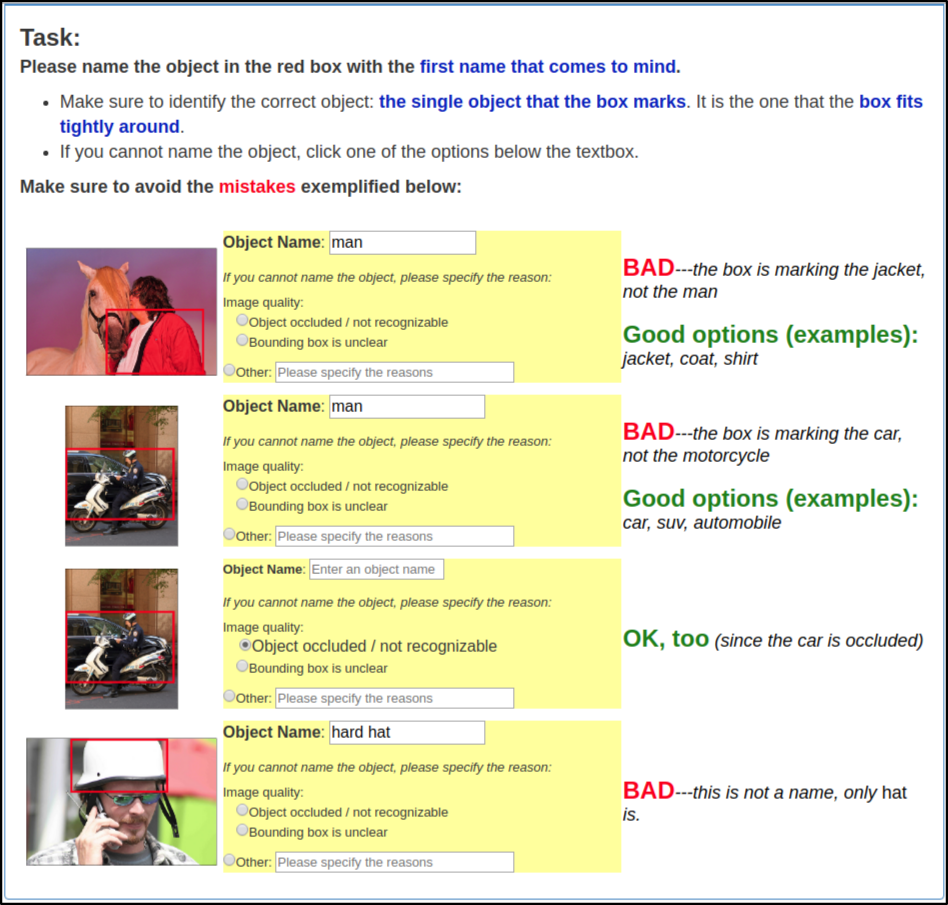
\includegraphics[width=1.5\columnwidth]{figures/round0.png}
  \caption{Instructions for AMT annotators for the first round.}
  \label{fig:instructions1}
\end{figure*}

\begin{figure*}[htp]
  \centering
  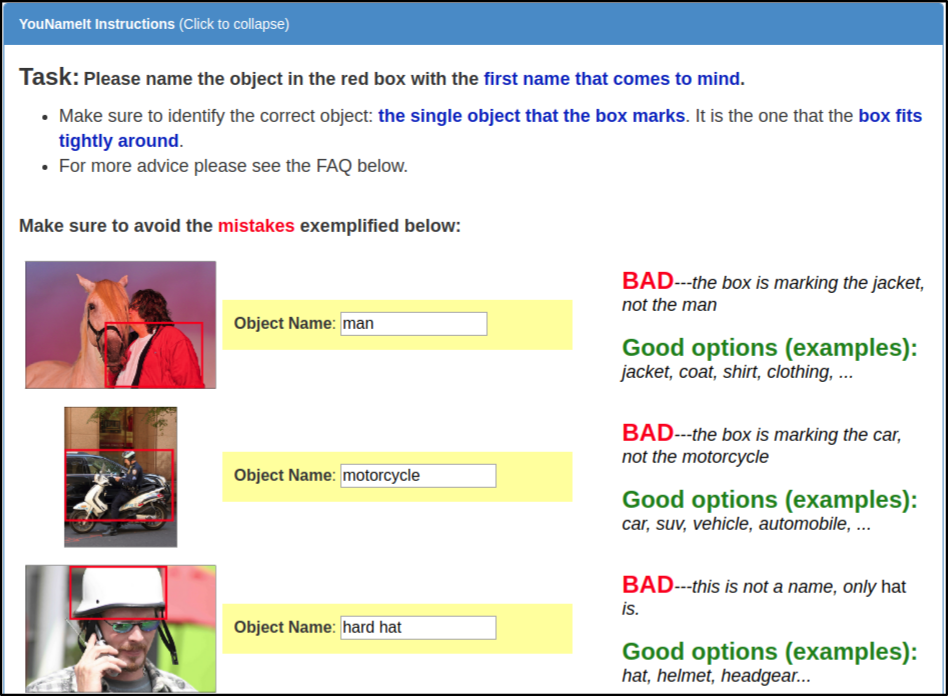
\includegraphics[width=1.5\columnwidth]{figures/round1+_p1.png}
  \caption{Instructions for AMT annotators for rounds~$2$ to~$4$. They were accompanied by the FAQ in Figure~\ref{fig:faq}}
  \label{fig:instructions2}
\end{figure*}
%
\begin{figure*}[htp]
  \centering
  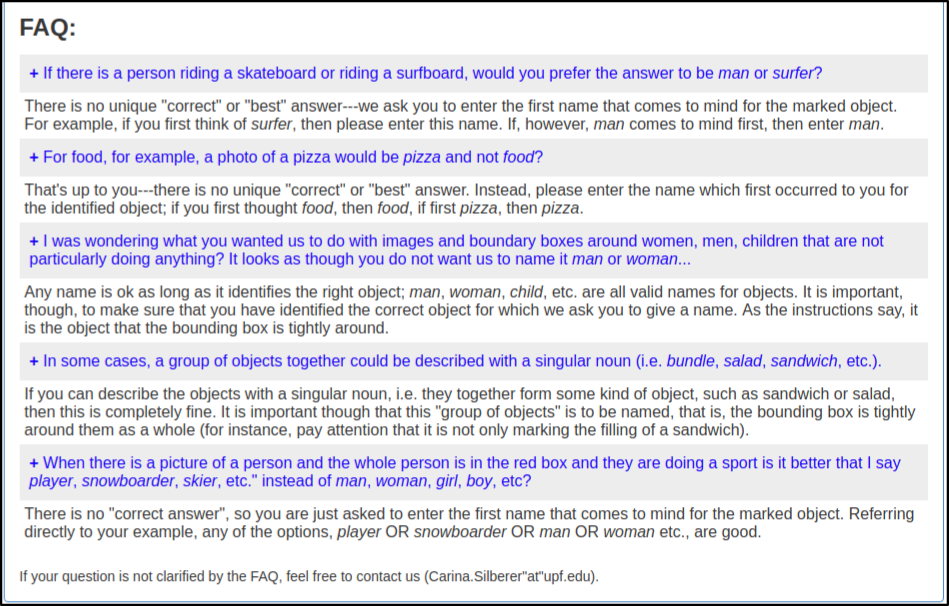
\includegraphics[width=1.5\columnwidth]{figures/round1+_p2.png}
  \caption{FAQ accompanying the instructions for AMT annotators for rounds~$2$ to~$4$.}
  \label{fig:faq}
\end{figure*}




\end{document}


%%% Local Variables:
%%% mode: latex
%%% TeX-master: t
%%% End:
